\documentclass[11pt, a4j]{bthesis}

%-usepackage---------------------------------------%
\usepackage[dvips]{graphicx}
\usepackage{subfigure}
\usepackage{amsmath}
\usepackage{txfonts}
\usepackage{ascmac}
\usepackage{bm}
\usepackage{multirow}
\usepackage{textmf/drafts}
\usepackage{float}
\usepackage{url}
%-end usepackage-----------------------------------%

% 要旨用和文題目 英文題目
\AJtitle{マルチFPGAボードによるGoogLeNetの高速化}

% 要旨用和文題目 英文題目
\TJtitle{マルチFPGAボードによるGoogLeNetの高速化}

\Jauthor{飯塚 健介}
\Eauthor{Kensuke Iizuka}
\Kauthor{イイヅカ ケンスケ}
\StudentID{61401007}

\Boss{天野 英晴 教授}
\Tmajor{情報工学科}
\Amajor{情報工学}
\Emajor{Information and Computer Science}

%-review mode--------------------------------------%
%\pagestyle{drafts}
%\renewcommand{\baselinestretch}{1.5}
%-end review mode----------------------------------%

\begin{document}
\pagestyle{empty}

%-title--------------------------------------------%
\maketitle
%-end title----------------------------------------%


%-abstract-----------------------------------------%
\jabst{
    昨今,人工知能が最新技術のトレンドとして様々なメディアに取り上げられている.
    人工知能技術が組み込まれる自動運転,レコメンドシステム,自動翻訳などのサービスは日々の生活をより豊かにすると期待されている.
    人工知能技術を実現させる機械学習の中でも,画像認識や自然言語処理,物体検出などの分野で
    大きな貢献を果たしているニューラルネットワークは一躍注目されていて,研究開発が盛んに行われている.
    ニューラルネットワークの一種である畳み込みニューラルネットワーク(CNN: Convolutional Neural Network)は畳み込み演算を主な計算とする.
    CNNは認識精度向上を目指し様々なモデルが提案されているが
    % ここの部分をもっと充実させたい.
    年々その計算量が増加する傾向にあり,研究サイクルを早くする,データセンターでのアプリケーションとしての利用に耐えうる,
    高速化,電力性能向上が求められている.

    しかし,汎用プロセッサではその要求を満たすことができないので,各半導体メーカや研究機関は専用のアクセラレータの開発に取り組んでいる.
    日本でも国立研究開発法人新エネルギー・産業技術開発機構(NEDO)は
    「省電力AIエンジンと異種エンジン統合クラウドによる人工知能プラットフォーム」プロジェクトで
    複数のFPGA,GPU,メモリなどの異種ノードを多数接続した大規模計算基盤Flow-in-Clowd(FiC)を開発している.
    複数のFPGAは高機能スイッチノードとして多数の高速リンクが接続され,FiCの高速通信のスイッチングの役割を担う.
    このマルチFPGAシステムは主演算を行うGPUノードであるが,FPGAノードも余った計算資源を利用してAIエンジンとしての役割も担うことができる.
    本研究ではマルチFPGAシステムに2014年の国際画像認識コンペで最高精度をマークしたCNNモデルの1つであるGoogLeNetを実装し,評価した.
    % 性能でCPUの〇〇倍,GPUの〇〇倍を達成し電力効率でCPUの〇〇倍,GPUの〇〇倍を達成した.
}
\makejabstract
%-end abstract-------------------------------------%


%-contents-----------------------------------------%
\pagenumbering{roman}
\tableofcontents
\listoffigures
\listoftables
%-end contents-------------------------------------%


%-body---------------------------------------------%
\pagestyle{headings}
\pagebreak
\pagenumbering{arabic}
\setcounter{page}{1}

\chapter{序論}
{
    \label{chap:introducion}

    \section{本研究の背景}
    \label{sec:backgroud}
    人工知能と称される機械学習をベースにした技術は爆発的な普及を見せていて日夜,メディアで取り上げられるだけでなく,
    自動運転やスマートスピーカー,スマートフォン向けアプリケーションなど様々なシステムに取り込まれている.
    しかし,人工知能のさらなる普及にはその計算基盤が必要である.
    その中でも特に画像認識や物体検出などの分野で活躍する畳み込みニューラルネットワーク(CNN)はその計算の特性から
    汎用CPUでは効率よく演算処理ができない.インテルやNVDIAなど大手半導体メーカーを始めとしてGoogleやMicrsoftなども
    人工知能向け専用アクセラレータの開発に心血を注いでいる.
    各社,研究機関はGPU,ASIC,FPGAなど様々なデバイス,手法で高速化を図る.
    その中でもFPGAはその電力効率のよさ,開発周期の短さ,再構成可能であることから注目され研究がなされている.
    日本でも国立研究開発法人新エネルギー・産業技術開発機構(NEDO)は「省電力AIエンジンと異種エンジン統合クラウドによる人工知能プラットフォーム」と銘打ったプロジェクトで
    複数のFPGA,GPU,メモリなどの異種ノードを多数接続した大規模人工知能計算基盤Flow-in-Clowd(FiC)を開発している.
    このFiCはデータセンターなどに導入されるクラウドシステムである.主演算装置となる複数のGPUを複数のFPGAのスイッチノードに接続し,
    高速通信を行う.高機能スイッチノードととなるマルチFPGAは多数の高速リンクが接続され,FiCの高速通信のスイッチングの役割を担う.
    さらにこのマルチFPGAシステムはスイッチノードという役割に加え,AIエンジンとしての役割も担う.
    そこで本研究ではマルチFPGAシステムの試作ボードであるFiC-SW1を複数枚用いて,CNNのモデルであるGoogLeNetを実装し,評価を取った.

    \section{研究目的}
    \label{sec:purpose}
    本研究の目的はマルチFPGAシステム上にGoogLeNetを実装し,既存研究や汎用CPU,GPUに対して
    性能向上を目指すことである

    \section{本論文の構成}
    \label{sec:composition}
    \ref{chap:googlenet}章では実装対象であるGoogLeNetと畳込みニューラルネットワークの概要を説明する.
    \ref{chap:ficsw}章では本研究で用いるマルチFPGAシステムとそのプロジェクトの概要を紹介する.
    \ref{chap:survey}章では本研究に関連する先行研究について説明する.
    \ref{chap:parallel}章ではGoogLeNetの並列化手法について説明する.
    \ref{chap:implement}章では\ref{chap:paralell}での並列化を考慮した実装方法について説明する. 
    \ref{chap:eval}章では本研究の評価を行う. 
    \ref{chap:conclusion}では本論文の結論を述べる.
}


\chapter{CMOS VLSIにおける電力とSOTB技術}
{
\label{chap:vlsi}
\section{消費電力}
\label{sec:power}
半導体技術の向上により集積度の高い集積化路が広く用いられるようになった。集積度の高い集積化路をVLSI(Very Large Scale Integration)と呼ぶ。VLSIでは何十万以上ものトランジスタが1チップ上に搭載されている。集積度を向上させることにより高い性能を実現する一方で、その主な問題は消費電力の増加であった。そのような背景から現在ではnMOSトランジスタとpMOSトランジスタを相補的に組み合わせて構成するCMOSプロセスが広く使われている。一般にCMOSを用いたVLSIの電力消費は2つの要素に分けることができる。
\begin{itemize}
\item ダイナミック消費電力$P_{dynamic}$
\item スタティック消費電力$P_{static}$
\end{itemize}

つまり、全体の消費電力$P_{total}$との関係は
\begin{eqnarray}
P_{total} = P_{dynamic} + P_{static}
\end{eqnarray}
である。
\subsection{ダイナミック電力}
\label{subsec:dynamic_power}
ダイナミック電力の要因は以下の2種類に分類できる。
\begin{itemize}
\item ゲートのスイッチングにより発生する負荷容量への充放電
\item pMOSとnMOSが同時にオンとなることにより発生する貫通電流
\end{itemize}
ただし大部分のダイナミック電力は前者のスイッチング電力である。このスイッチング電力を$P_{switching}$とすると以下の式で表される。\cite{west}
\begin{eqnarray}
P_{switching} = \alpha C V^2_{DD}f
\end{eqnarray}
ここで$\alpha$は活性化率と呼ばれ回路中で0から1へ遷移する確率、$C$は負荷容量、$V_{DD}$は電源電圧である。

\subsection{グリッチ}
\label{subsec:glitch}
直列に回路を接続する構造の場合、グリッチと呼ばれる信号変化により発生する電力を考慮する必要がある。グリッチによる信号変化は本来不要なものであるがビット間の遅延時間の差により発生してしまう。図\ref{fig:glitch}はCMAのPEにおいて積算を行った時の波形である。左の赤い線が演算が開始した時刻であり、右の赤い線が演算の完了時刻を表している。最終的な値に確定するまでの間に不要なスイッチングが発生しているのが確認できる。組み合わせ回路の規模が大きくなり、複雑化すれほどグリッチの影響は大きくなる。このグリッチによる消費電力は全体の消費電力の40\%以上を占めることもあり、グリッチを取り除くことが消費電力削減に有効である。\cite{glitch}

\begin{figure}[h]
\centering
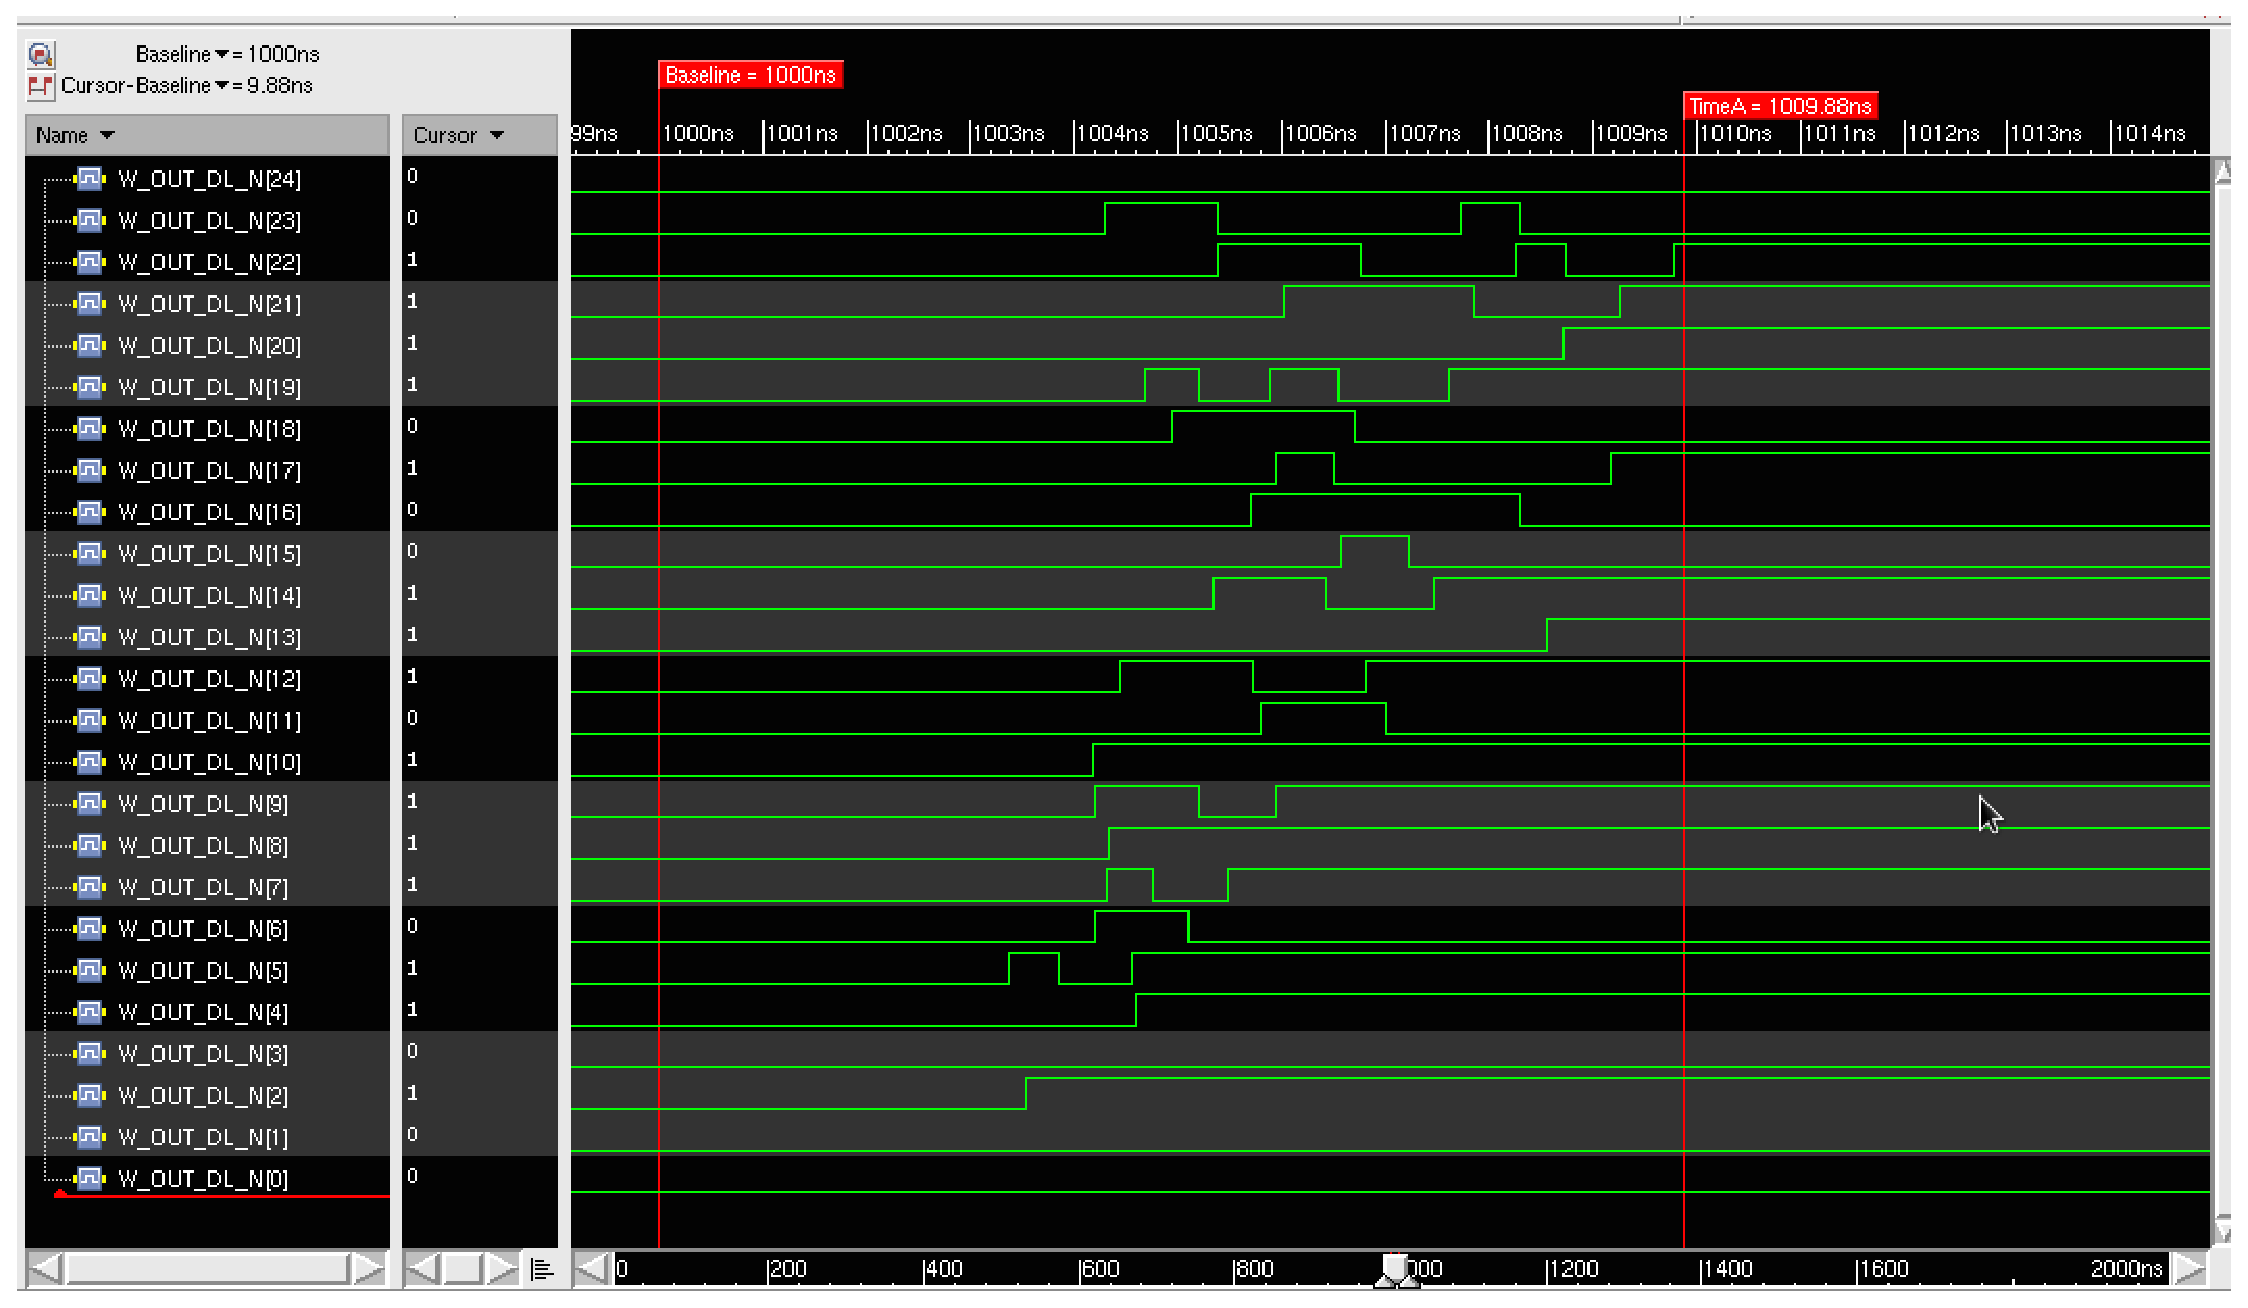
\includegraphics[width=12cm]{./chap2/fig/glitch.eps}
\caption{グリッチの様子}
\label{fig:glitch}
\end{figure}

\subsection{スタティック電力}
\label{subsec:static_power}
スタティック電力はスイッチングしていないときにも消費される電力である。スイッチングしていないときに流れる電流をリーク電流と呼び。その原因はゲート絶縁膜をキャリアが通過することによるゲートリーク電流や、サブスレッショルドリーク電流など様々である。リーク電流を$I_{leak}$とするとスタティック電力$P_{static}$は以下のように表される。
\begin{eqnarray}
P_{static} = I_{leak}V_{DD}
\end{eqnarray}


\section{SOTB技術}
\label{sec:sotb}
\subsection{SOTBの特徴}
SOTB(Silicon on Thin Buried Oxide)は超低電力あるデバイス技術研究組合(LEAP)によって開発されたSOI\footnote{SOI: Sillicon on Insulator}
}の一種である。10nm程度の極薄のSOI層とBOX層\footnote{BOX:Buried Oxide}がウェル基盤の上に積層されている。標準的なバルクCMOSテクノロジでは微細化に伴いスレッショルド電圧のばらつきなどの特性のばらつきが問題であった。SOTBは特性ばらつきが小さくバルクと比べて半分程度のばらつきに抑制されている。\cite{sotb_variability}これによりスレッショルド電圧を下げることが可能となり、低電力で動作させることが可能となる。さらに、BOX層の下のウェル基盤に電圧を印加することによりリーク電流を制御することが可能である。この印加する電圧をボディバイアス電圧と呼び、ボディバイアス電圧を制御することによりリーク電力を最適化することができる。

\subsection{SOTBトランジスタの構造}
図\ref{fig:sotb}にSOTBトランジスタの構造を示す。\cite{sotb_book}
\begin{figure}[h]
\centering
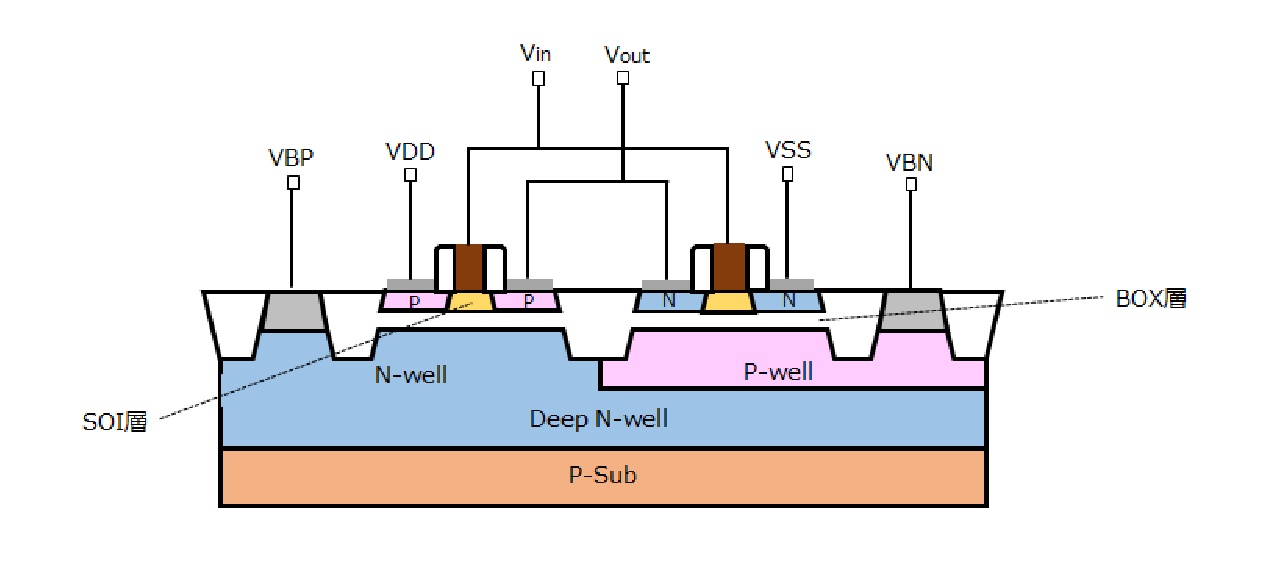
\includegraphics[width=12cm]{./chap2/fig/sotb.eps}
\caption{SOTBトランジスタの構造}
\label{fig:sotb}
\end{figure}
\subsection{ボディバイアス制御}
ボディバイアス電圧のうちnMOS側の電圧を$V_{BN}$、pMOS側の電圧を$V_{PN}$、全体のボディバイアス電圧を$V_{BB}$と呼ぶこととする。nMOS、pMOSのバランスを揃える場合以下の関係が成り立つ。
\begin{eqnarray}
VBN & = & VBB \\
VBP & = & VDD - VBB
\end{eqnarray}

$V_{BB}$の値が負のときをリバースボディバイアス、0のときゼロバイアス、正のときをフォワードボディバイアスと呼び以下のトレードオフがある。
\begin{itemize}
\item リバースボディバイアス
	\begin{itemize}
	\item リーク電流が減少
	\item 遅延時間が増加
	\end{itemize}
\item フォワードボディバイアス
	\begin{itemize}
	\item リーク電流が増加
	\item 遅延時間の減少
	\end{itemize}
\end{itemize}

ボディバイアスの制御とは上記のような性能と電力のバランスを制御することである。

\chapter{関連研究}
{
\label{chap:survey}
}
\chapter{Valiable Pipelined CMAの概要}
{
\label{chap:vpcma}
本章では、本論文で対象としているアーキテクチャであるValiable Pipelined CMAの概要を説明する。
\section{CMAの概要}
\label{sec:about_cma}
CMAは主にバッテリー駆動の組み込みシステムにおけるマルチメディア処理を行うアクセラレータとして提案された。\cite{cma_micro}マルチメディア処理の特性として一定時間内に一定量のデータ処理を行うことが要求される。一方でこれらの処理を要求されている時間よりも早く完了させることによって得られる利益は少ない。したがって、処理時間を調整して不必要な消費電力を削減することが可能であり、バッテリー使用時間を長くすることにつながる。CMAアーキテクチャでは主に以下のコンセプトによって消費電力の削減を図っている。

\begin{itemize}
\item PEアレイからクロックツリーとレジスタを除去し、完全な組み合わせ回路として構成する
\item 各PEの演算やデータパスの動的な再構成を行わない
\end{itemize}

一般的なDRPでは、動的な再構成のために各PEにおいてレジスタを持ち、クロックが供給される。したがってクロックツリーと動的な再構成のための処理において大きな電力を消費する。一方でCMAではPEにはレジスタやクロックツリーは存在せず組み合わせ回路のみで構成している。このような構成を採用することにより上記のコンセプトを実現している。

初代試作機のCMA-1からCCSOTBまではPE\_ARRAYへのクロック供給とレジスタはなかった。そこでPE\_ARRAYをパイプライン分割することによる発生するオーバーヘッドと性能の関係が研究されValiable Pipelined CMAが提案された。\cite{vpcma}パイプライン分割のためにPE\_ARRAYに追加されたパイプラインレジスタにおける消費電力は全体の数\%であり、クロックツリーでの消費電力は最大で全体の60\%を占めている。
このようにパイプライン分割による電力増加がある、一方で高いスループット向上が得られ全体としてはエネルギー効率が改善されている。エネルギー効率は最大で96\%向上したと報告されている。
% ところが、パイプライン分割による性能向上の影響が勝り、最大で96\%のエネルギー効率を実現できることが確認された。

% %DRPとCMAの構成図
% \begin{figure}[h]
%   \begin{center}
%     \begin{tabular}{c}

%       % 1
%       \begin{minipage}{0.33\hsize}
%         \begin{center}
%           %\includegraphics[clip, width=4.5cm]{./fig/DRP.eps}
%           \hspace{1.6cm} (a)DRPにおけるPEの構成
%         \end{center}
%       \end{minipage}

%       % 2
%       \begin{minipage}{0.33\hsize}
%         \begin{center}
%           %\includegraphics[clip, width=4.5cm]{./fig/PE.eps}
%           \hspace{1.6cm} (b)CMAにおけるPEの構成
%         \end{center}
%       \end{minipage}


%     \end{tabular}
%     \caption{DRPとCMAにおける構成の違い}
%     \label{fig:DRP_vs_CMA}
%   \end{center}
% \end{figure}


\section{CMAの構成}
\label{sec:about_cma}
CMAを構成する要素とそれらの動作を説明していく。CMAは主に以下の要素で構成されている。
\begin{itemize}
\item PE\_ARRAY    
\item $\mu$コントローラ
\item コンフィギュレーションレジスタ
\item 定数値レジスタ
\end{itemize}

\subsection{PE\_ARRAY}
\label{subsec:pe_array}
図\ref{fig:pe_array}にPE\_ARRAYの構成を示す。12列$\times$8行のPEとそれらの相互接続、パイプライン分割のためのレジスタから構成されている。パイプラインレジスタはPEの行と行の間に置かれている。パイプラインの動作に関しては\ref{subsec:pipeline}節で詳しく説明する。すでに述べているようにPEに対してはクロックの分配をしない、一方でパイプラインレジスタへはクロックが分配されている。ただし、可変パイプラインであるため使用しないパイプラインレジスタに対してはクロックゲーティングを行うことで不要な消費電力が発生しないようにしている。このPE\_ARRAY全体はおよそ0.5V$\sim$1.2Vの電源電圧で動作する。PE\_ARRAYの入出力は南方向のみであり、入力にはfetchレジスタが、出力にはgatherレジスタが接続されている。つまり、fetchレジスタ、gatcherレジスタともにPE\_ARRAYの0行目の0番から11番までの列と接続されている。そのためデータ幅は25bit$\times$12である。fetchレジスタにデータを書き込むことでPE\_ARRAYでの演算が開始し、適切なタイミングでgatherレジスタにデータを取り込む。\\

\begin{figure}[p]
\centering
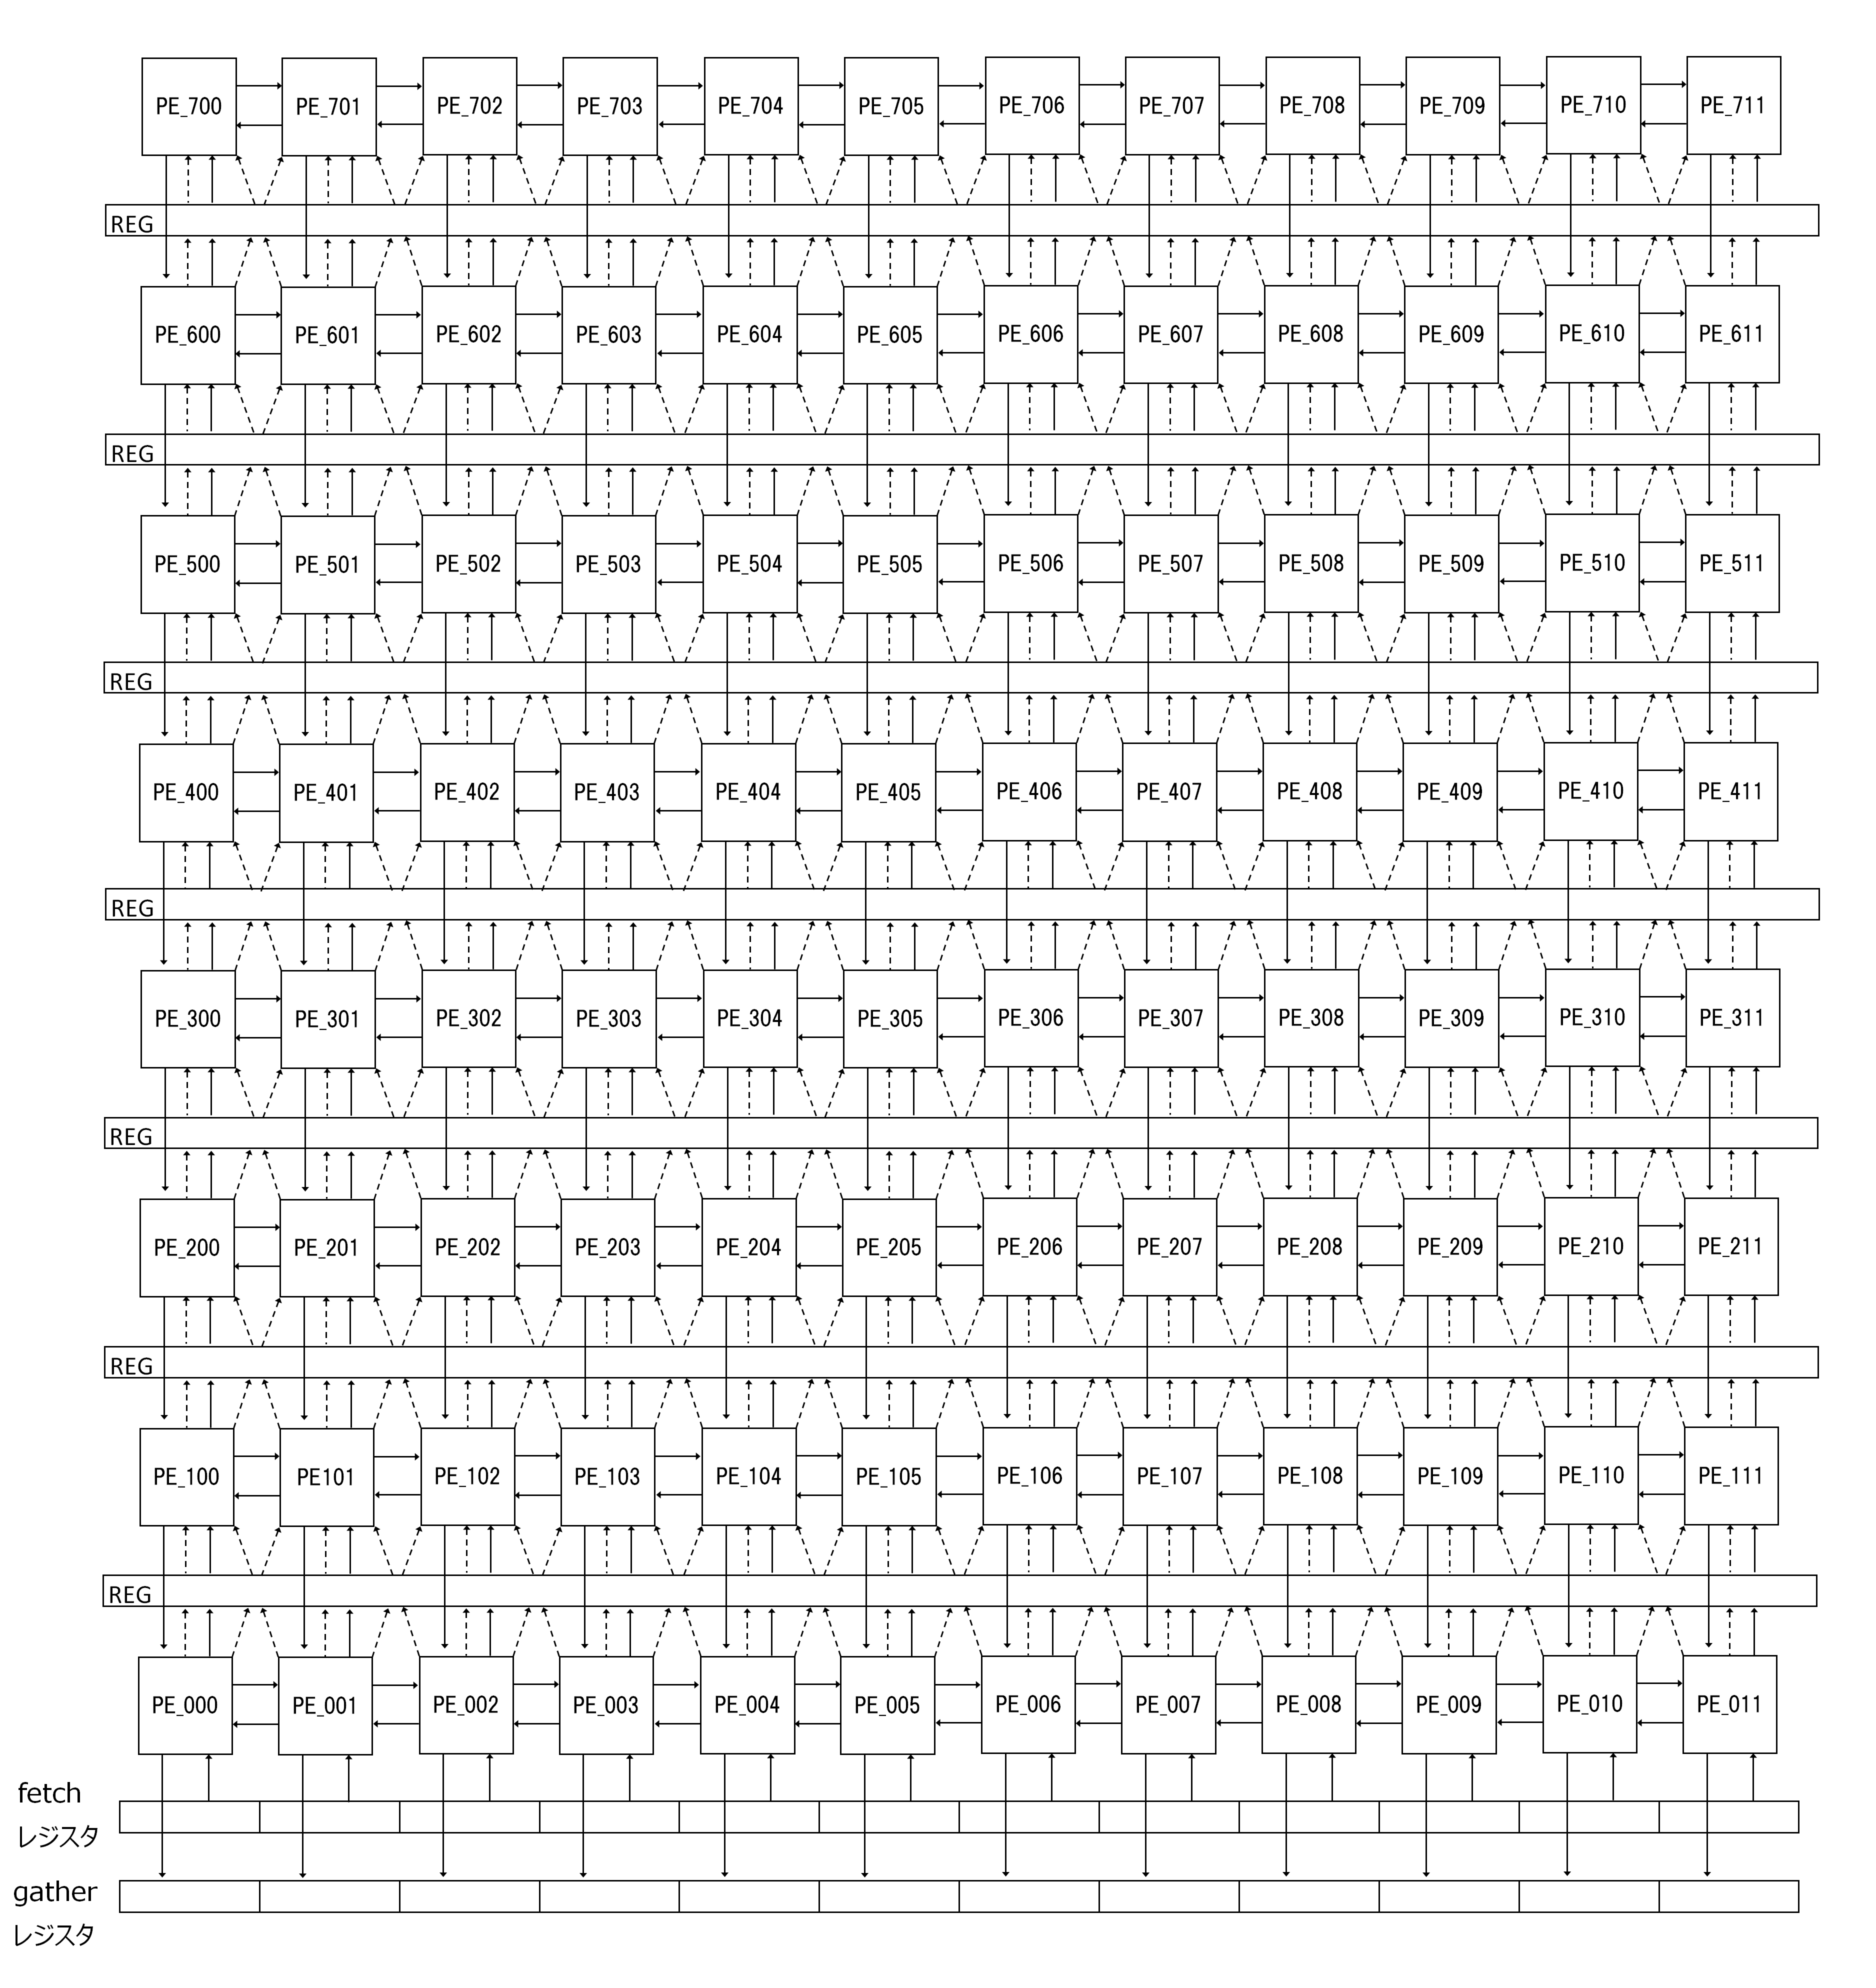
\includegraphics[scale=0.15]{./chap4/fig/PE_ARRAY.eps}
\caption{PE\_ARRAYの構成}
\label{fig:pe_array}
\end{figure}

PEの構成を図\ref{fig:pe}に示す。各PEは以下の要素から構成されている。
\begin{itemize}
\item ALU(Arithmetic Logic Unit)
\item ALUへの入力のセレクタ
\item SE(Switch Element)
\end{itemize}

\begin{figure}[h]
\centering
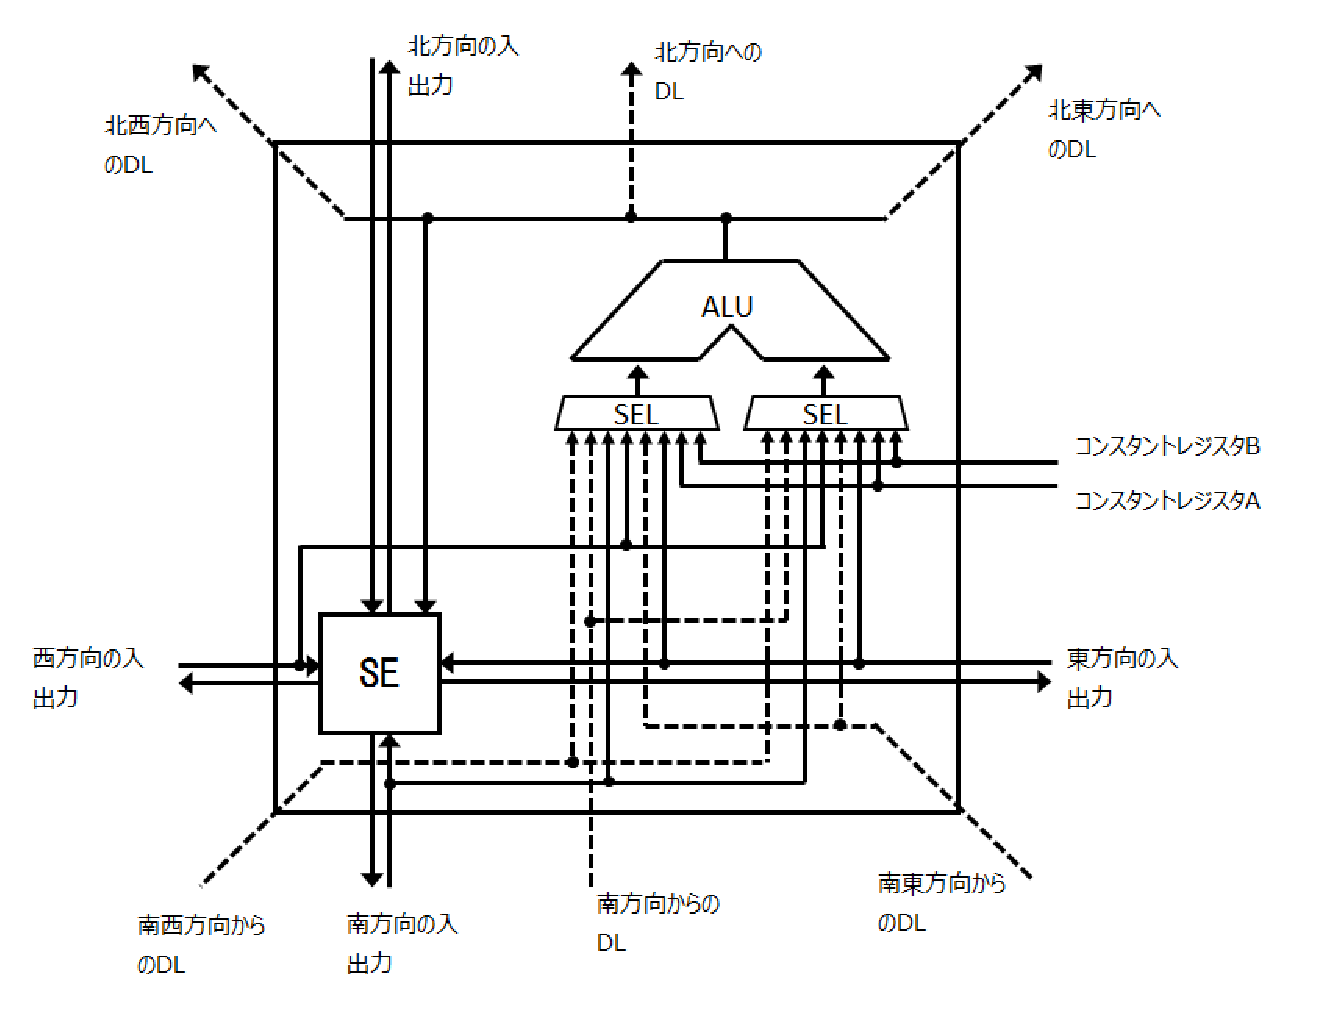
\includegraphics[scale=0.5]{./chap4/fig/PE_detail.eps}
\\ \begin{flushleft}※DL:ダイレクトリンク\end{flushleft}
\caption{PEの構成}
\label{fig:pe}
\end{figure}

ALUはデータ幅25bitの2入力1出力で演算を行う部分である。ALUの出力はSEへの入力、隣接する北方向、北東方向、北西方向のPEへのダイレクトリンクへと接続される。ダイレクトリンクとはSEを経由せずに隣接するPEへデータを送るローカルな接続である。図\ref{fig:pe}において破線で表される接続がダイレクトリンクである。ALUで使用可能な演算を表\ref{table:ALU}に示す。ただし、入力される2つのデータを$indataA$, $indataB$としている。SEは東西南北方向の隣接するPEとの相互接続を行うスイッチである。ALUへの入力のセレクタは東西南方向からの入力、南方向、南東方向、南西方向からのダイレクトリンク、および定数値レジスタから演算に使用するデータを選択する。図\ref{fig:pe_array}においてPE間の相互接続を見ると行をまたぐ接続ー3つのダイレクトリンク、北方向の出力と出力、南方向からの入力ーはパイプラインレジスタを経由することがわかる。ただし、南方向への出力、北方向からの入力はパイプラインレジスタを経由していない。

\begin{table}[h]
\centering
\caption{ALUで使用可能な演算の一覧}
\label{table:ALU}
\begin{tabular}{|c|l|} \hline
演算名 & 出力される演算結果 \\ \hline \hline
NOP & 0 \\ \hline
ADD &  $indataA$ + $indataB$\\ \hline
SUB &  $indataA$ - $indataB$\\ \hline
MULT & $indataA$ $\times$ $indataB$ \\ \hline
SL & $indataA$を$indataB$ビット左へシフト \\ \hline
SR &  $indataA$を$indataB$ビット右へ論理シフト\\ \hline
SRA & $indataA$を$indataB$ビット右へ算術シフト \\ \hline
\multirow{2}{*}{SEL} & if ($indataA$のMSB==1) $indataA$ \\
					&  else \hspace{89pt} $indataB$ \\ \hline
CAT & $indataA$ \\ \hline
NOT & NOT $indataA$ \\ \hline
AND &  $indataA$ AND $indataB$\\ \hline
OR &  $indataA$ OR $indataB$\\ \hline
XOR & $indataA$ XOR $indataB$ \\ \hline
\multirow{2}{*}{EQL} & if ($indataA$==$indataB$) $indataA$ \\
					&  else \hspace{80pt} $indataB$ \\ \hline
\multirow{2}{*}{GT} & if ($indataA$ $>$ $indataB$) $indataA$ \\
					&  else \hspace{80pt} $indataB$ \\ \hline
\multirow{2}{*}{LT} & if ($indataA$ $<$ $indataB$) $indataA$ \\
					&  else \hspace{80pt} $indataB$ \\ \hline
\end{tabular}
\end{table}

\subsection{$\mu$コントローラ}
\label{subsec:micro_controller}
$\mu$コントローラは固定長16bitの命令を実行する小さなプロセッサであり、PE\_ARRAYとデータメモリの間のデータ転送などを行う。$\mu$コントローラには表\ref{table:iset}に示す命令セットを持つ。$\mu$コントローラは25bitの汎用レジスタを16個持っている。表\ref{table:iset}中のrd,rsはレジスタを表す。n,imm,adr, X, X1, X2は即値であり、左の()で囲まれた数値はビット数である。

\begin{table}[p]
\begin{center}
\caption{$\mu$コントローラの命令セット}
\label{table:iset}
\begin{tabular}{|l|l|l|} \hline
オペコード & オペランド & 命令の意味 \\ \hline
NOP & & \\ \hline
ADD & rd, rd & rd $\leftarrow$rd + rs \\ \hline
SUB & rd, rs & rd $\leftarrow$rd - rs \\ \hline
MV & rd, rs & rd $\leftarrow$ rs\\ \hline
DONE & & プログラムの終了を示す\\ \hline
DELAY & n(4) & G.Rにデータを取り込むまでの遅延サイクル数nを指定する \\ \hline
LDI & rd, imm(8) & rd $\leftarrow$  imm \\ \hline
ADDI & rd, imm(8) & rd $\leftarrow$ rd  + imm \\ \hline
BEZ & rd, imm(8) & if (rd==0) pc $\leftarrow$ pc + imm \\ \hline
\multirow{2}{*}{BEZD} & \multirow{2}{*}{rd, imm(8)} & rd $\leftarrow$ rd - 1 \\
& &  if (rd==0) pc $\leftarrow$ pc + imm \\ \hline
BNZ & rd, imm(8) & if (rd!=0) pc $\leftarrow$ pc + imm \\ \hline
\multirow{2}{*}{BNZD} & \multirow{2}{*}{rd, imm(8)} &  rd $\leftarrow$ rd - 1\\ 
& & if (rd!=0) pc $\leftarrow$ pc + imm \\ \hline
& & データメモリからF.Rへのデータをロードする際の設定を行う \\
LD\_SET & adr(8), X(4) &  adr: データメモリのロード開始アドレスを指定 \\
& & X:データマニピュレータのテーブル番号を指定\\ \hline
& & G.Rからデータメモリへデータをストアする際の設定を行う \\
ST\_SET & adr(8) , X(4) &  adr: データメモリのストア開始アドレスを指定\\ 
& & X: データマニピュレータのテーブル番号を指定\\ \hline
\multirow{6}{*}{LDST\_ADD} &  \multirow{6}{*}{X1(4), X2(4)} & データメモリのロード開始アドレスからX1個のデータを \\
& & 						F.Rレジスタへロードする \\
& & 						ロード開始アドレスにX1を加算する \\
& & 						 nサイクルの遅延の後G.Rからデータメモリのストア開始アドレス \\
& & 						からX2個のデータをストア \\
& & 						ストア開始アドレスをX2加算する\\ \hline
\end{tabular}
\end{center}
※F.R: fetchレジスタ G.R: gatherレジスタ pc: プログラムカウンタ
\end{table}

データメモリのロードとストアの動作について説明する。$\mu$コントローラにおけるデータメモリは12個のバンクに分割されている。そのため同時に25bitのデータを最大で12個読み書きすることが可能である。これはPE\_ARRAYが12列で構成されているためである。データメモリからロードしたデータをfetchレジスタのどの列へ書き込みを行うかの対応付けを行うのがデータマニピュレータである。同様にgatherレジスタのどの位置からデータを読み込み、データメモリへストアするかの対応付けをデータマニピュレータが行う。

表\ref{table:ldtbl}をデータマニピュレータのテーブルとして指定した時のロード時の様子を図\ref{fig:LD_dmanu}に示す。マスク部分はその列番号についてロードを行うか否かを表している。0の列のfetchレジスタには書き込みをせず、1の列のfetchレジスタに対して書き込みを行う。fetchレジスタへ書き込みを行う列はデータメモリのアドレスを指定する必要がある。LDテーブルは各列についてロード開始アドレスに対するオフセットを持っており、これによって読み込むデータのアドレスを指定している。この例ではロードするデータの数は4個であるため、1回のロードが終わるとロード開始アドレスは4加算され次のロード処理に備える。この機構によりPE\_ARRAYとデータメモリのやり取りを柔軟に行うことが可能となる。

\begin{table}[h]
\centering
\caption{LDテーブルの例}
\label{table:ldtbl}
\begin{tabular}{|c|c|c|c|c|c|c|c|c|c|c|c|c|} \hline
fetchレジスタの列番号 & 0 & 1 & 2 & 3 & 4 & 5 & 6 & 7 & 8 & 9 & 10 & 11 \\ \hline \hline 
マスク部分 & 1 & 0 & 0 & 1 & 0 & 0 & 1 & 0 & 0  & 1 & 0 & 0 \\ \hline
ロード開始アドレスに & \multirow{2}{*}{0x0} & \multirow{2}{*}{0x0} & \multirow{2}{*}{0x0} & \multirow{2}{*}{0x1} & \multirow{2}{*}{0x0} & \multirow{2}{*}{0x0} & \multirow{2}{*}{0x2} & \multirow{2}{*}{0x0} & \multirow{2}{*}{0x0} & \multirow{2}{*}{0x3} & \multirow{2}{*}{0x0} & \multirow{2}{*}{0x0} \\ 
対するオフセット & & & & & & & & & & & & \\ \hline
\end{tabular}
\end{table}

\begin{figure}[]
\centering
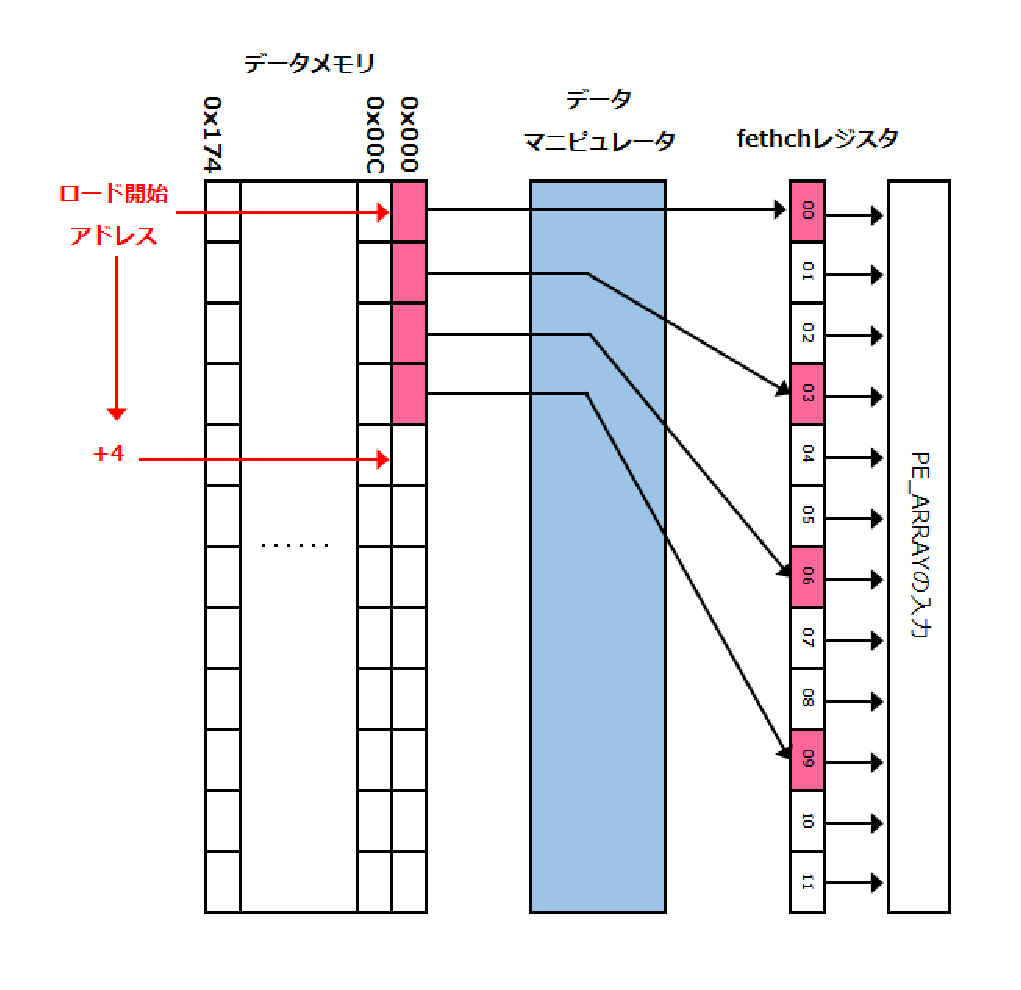
\includegraphics[width=8cm]{./chap4/fig/LD_dmanu.eps}
\caption{ロード時のデータマニピュレータ様子}
\label{fig:LD_dmanu}
\end{figure}


gatherレジスタへ演算結果を取り込みデータメモリへのストアが行われるのは表\ref{table:iset}で見たようにデータメモリからfetchレジスタへデータをロードしてから指定したサイクル数遅延してから行われる。これはPE\_ARRAYは大規模な組み合わせ回路であり計算結果が出力されるまでに長い時間が必要であり、$\mu$コントローラの1クロックサイクル以内に演算を完了できない場合が殆どだからである。ストアの動作に関しても同様にデータマニピュレータの対応付けによって指定した列の出力のみをデータメモリへ書き込み、書き込んだデータ数の分だけストア開始アドレスが加算される。表\ref{table:sttbl}をデータマニピュレータのテーブルとして指定した時のストア時の様子を図\ref{fig:ST_dmanu}に示す。この例ではストアするデータの数は2個であるため、1回のストアが終わるとストア開始アドレスは2加算される。

\begin{table}[h]
\centering
\caption{STテーブルの例}
\label{table:sttbl}
\begin{tabular}{|c|c|c|c|c|c|c|c|c|c|c|c|c|} \hline
gatherレジスタの列番号 & 0 & 1 & 2 & 3 & 4 & 5 & 6 & 7 & 8 & 9 & 10 & 11 \\ \hline \hline
マスク部分 & 1 & 0 & 0 & 0 & 0 & 0 & 1 & 0 & 0  & 0 & 0 & 0 \\ \hline
ストア開始アドレスに & \multirow{2}{*}{0x0} & \multirow{2}{*}{0x0} & \multirow{2}{*}{0x0} & \multirow{2}{*}{0x0} & \multirow{2}{*}{0x0} & \multirow{2}{*}{0x0} & \multirow{2}{*}{0x1} & \multirow{2}{*}{0x0} & \multirow{2}{*}{0x0} & \multirow{2}{*}{0x0} & \multirow{2}{*}{0x0} & \multirow{2}{*}{0x0} \\ 
対するオフセット & & & & & & & & & & & & \\ \hline
\end{tabular}
\end{table}

\begin{figure}[h]
\centering
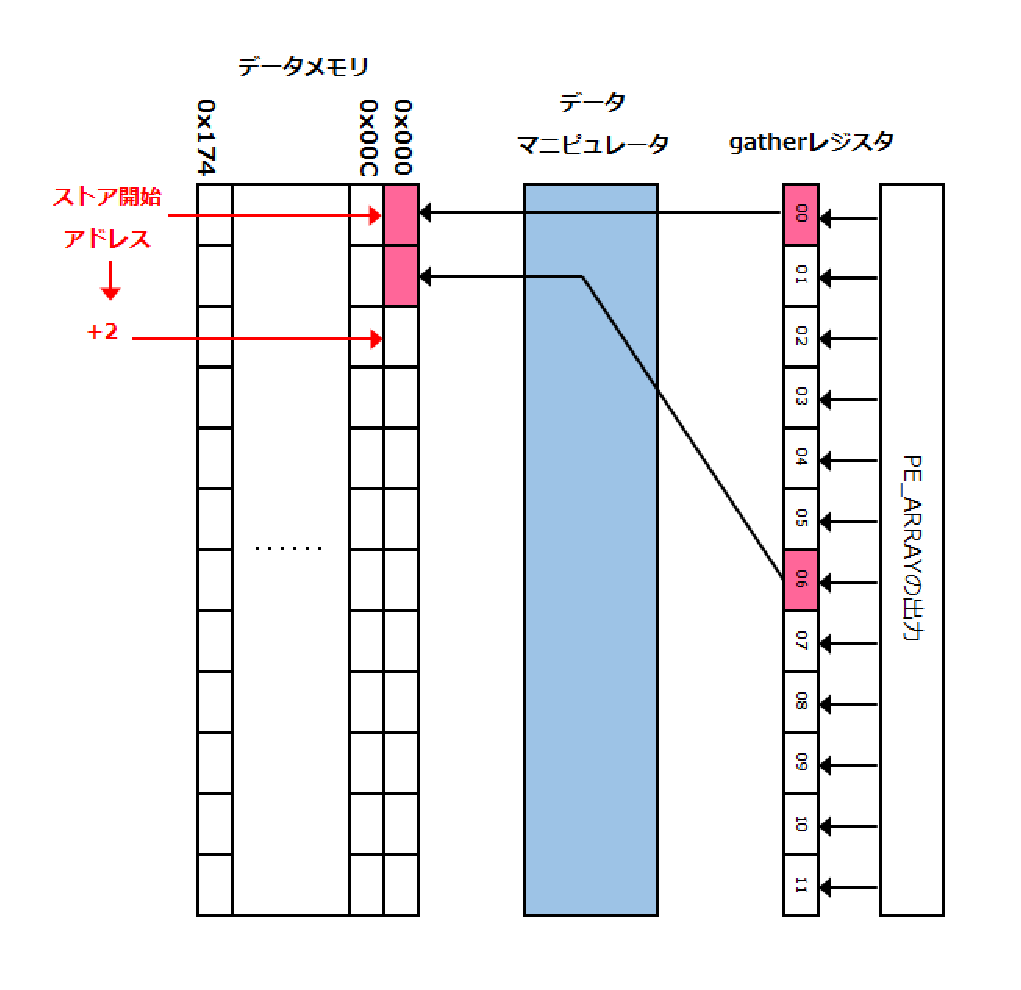
\includegraphics[width=8cm]{./chap4/fig/ST_dmanu.eps}
\caption{ストア時のデータマニピュレータの様子}
\label{fig:ST_dmanu}
\end{figure}


\subsection{コンフィギュレーションデータ}
\label{subsec:config_data}

コンフィギュレーションデータとはPE\_ARRAY内にある各PEとパイプラインレジスタの構成情報を指定するものである。PE\_ARRAYの外部にコンフィギュレーションレジスタが配置されており、そこからPE\_ARRAYへ送信される。使用するパイプラインレジスタをコンフィギュレーションデータに含めることでアプリケーションごとに可変なパイプライン段数を使用することが可能となる。すでに述べているようにアプリケーション実行を通してコンフィギュレーションデータは動的に変化することはない。

\section{演算のマッピングとアプリケーション実行の様子}
\label{sec:mapping}
PE\_ARRAYにアプリケーションをマッピングして実行する様子を説明する。前半ではパイプライン分割を行わない場合を、後半ではパイプライン分割を行った場合の動作を説明する。例としてRGB24bitのグレースケールを行うアプリケーションを用いる。PE\_ARRAYは12列あるがここでは簡略化のためにPE\_ARRAYのはじめの2列のみを示す。演算のマッピングされたPEとその相互接続の様子を図\ref{fig:mapping}に示す。各PEにマッピングされた演算が記されている。何も書かれたいない2つのPEはスイッチとしてのみ利用されていて、ALUは使用されない。

\begin{figure}[p]
\centering
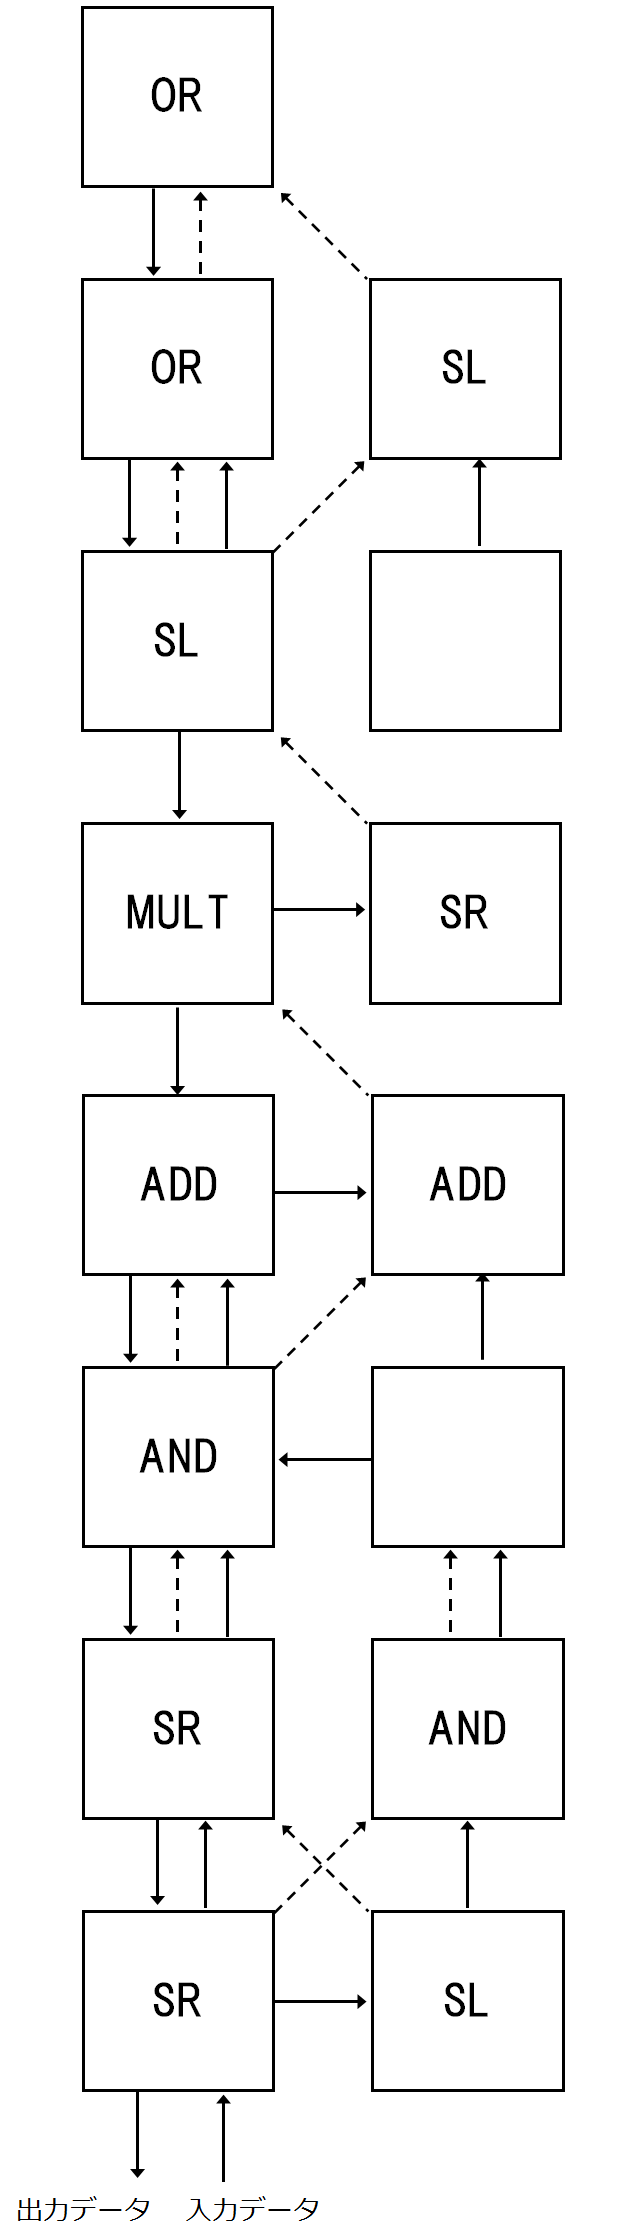
\includegraphics[width=4cm]{./chap4/fig/mapping.eps}
\caption{アプリケーションのマッピング例:}
\label{fig:mapping}
\end{figure}

次に$\mu$コントローラにおけるアプリケーション実行の様子を説明する。比較のためにパイプライン分割しない場合と、パイプライン分割する場合で同じクロックサイクル、つまり同じ周波数で動作する例を考える。

\subsection{パイプライン分割をしない場合}
\label{subsec:not_pipeline}
$\mu$コントローラにおける命令コードを以下に示す。この命令コードを実行したときの様子を図\ref{fig:not_pipelined_look}に示す。
\begin{itembox}[l]{パイプライン分割しない場合の命令コード}
\begin{verbatim}
        DELAY 7
        LDI r3,#8
        SET_LD #0,#6
        SET_ST #0x30,#6
LP:     LDST_ADD #0,#0
        NOP
        NOP
        NOP
        NOP
        NOP
        BNZD r3,LP
        DONE
\end{verbatim}
\end{itembox}

データメモリの0x0番地からデータを6個ロードして、データメモリの0x30番地にデータを6個ストアすることを8回ループすることを示している。演算終了まで7クロックサイクル遅延してからストアを行っている。演算結果をgatherレジスタに取り込むまでは新しいデータをPE\_ARRAYに入力して演算を開始させることができないのでそれまでNOP命令を挿入している。

\begin{figure}[h]
\centering
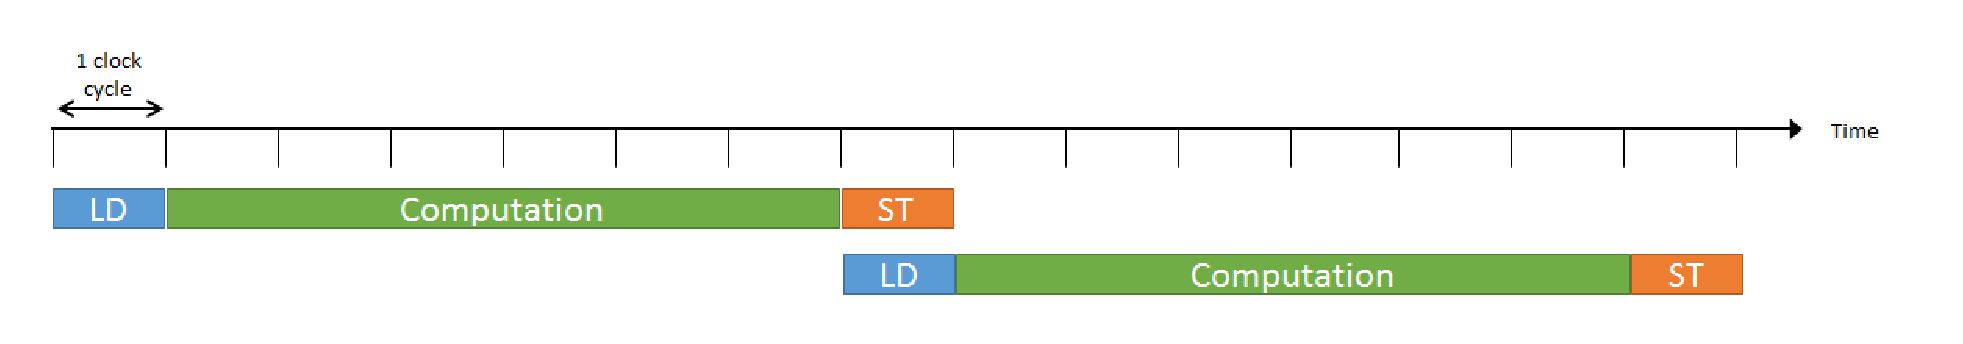
\includegraphics[width=12cm]{./chap4/fig/not_pipelined_look.eps}
\caption{パイプライン分割しない場合の実行の様子}
\label{fig:not_pipelined_look}
\end{figure}

\subsection{パイプライン分割をする場合}
\label{subsec:pipeline}
ここではすべてのパイプラインレジスタを用いる、すなわちパイプライン段数8の場合を考える。$\mu$コントローラにおける命令コードを以下に示す。この命令コードを実行したときの様子を図\ref{fig:pipelined_look}に示す。
\begin{itembox}[l]{パイプライン分割しない場合の命令コード}
\begin{verbatim}
        DELAY 7
        LDI r3,#8
        SET_LD #0,#6
        SET_ST #0x30,#6
LP:     LDST_ADD #0,#0
        BNZD r3,LP
        DONE
\end{verbatim}
\end{itembox}

\begin{figure}[h]
\centering
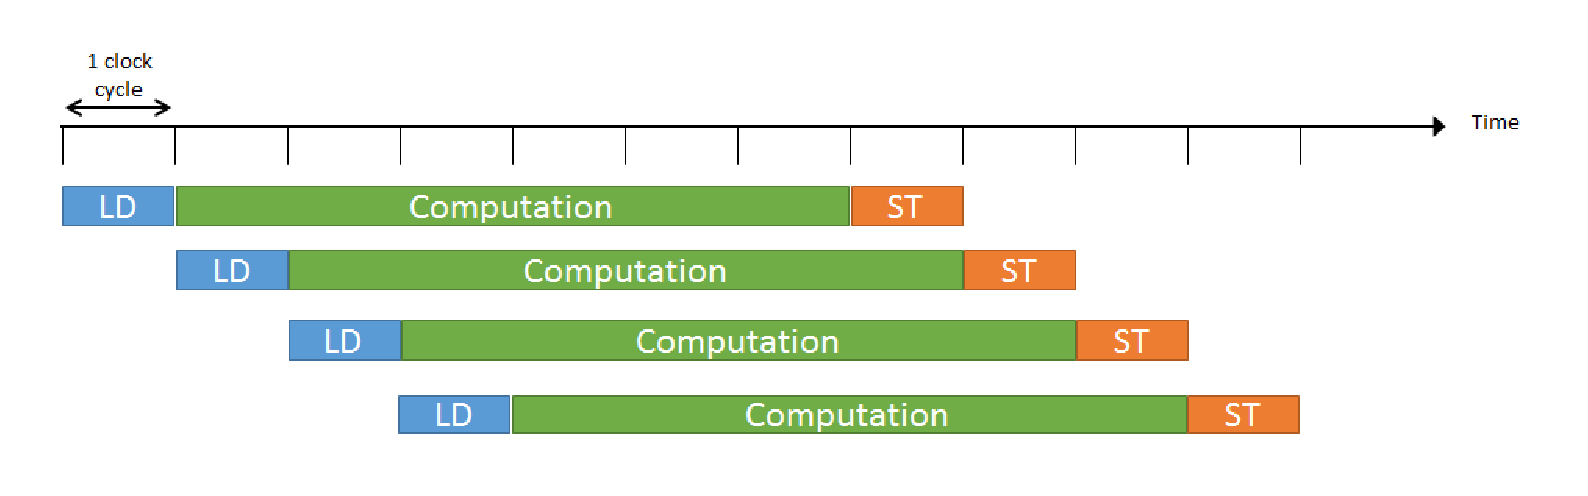
\includegraphics[width=12cm]{./chap4/fig/pipelined_look.eps}
\caption{パイプライン分割する場合の実行の様子}
\label{fig:pipelined_look}
\end{figure}

パイプライン分割しない場合の図\ref{fig:not_pipelined_look}と比べて各パイプラインステージで演算をオーバーラップさせて実行できることがわかる。

}

\chapter{パイプライン段数とボディバイアス制御による電力効率改善手法}
{
\label{chap:proposal}
Valiable Pipelined CMAはCCSOTBと比べて高い性能と高い電力効率が得られると示された。\cite{vpcma}一方で要求される性能が低い場合パイプライン分割のためのオーバーヘッドのためCCSOTBよりも高い電力となってしまうことが問題であった。この問題を解決するためにパイプライン分割とボディバイアス制御を同時を行うことを検討する。
\section{ボディバイアス電圧とパイプライン段数のトレードオフ}
\label{sec:trade_off}

ボディバイアス電圧を変化させると、遅延時間とリーク電力との間にトレードオフがあることは\ref{sec:sotb}節において述べた。つまり、動作周波数とリーク電力との間にトレードオフがある。パイプライン分割の段数を変化させることによるトレードオフについて説明する。パイプライン段数の増加により得られる利益は主に3つある。1つ目はPE\_ARRAYの長いデータパスを分割することで動作可能な周波数が高くなることである。2つ目はパイプラインレジスタを経由することにより\ref{subsec:glitch}節で述べたグリッチが次段のPEに伝搬するのを防ぐことが可能となることである。3つ目はオーバーラップして演算を進めることが可能となりスループットが向上することである。一方パイプライン段数の増加により発生する負の影響はクロックツリー、パイプラインレジスタでの消費電力が大きくなることである。

以上のトレードオフを表\ref{table:trade_off}にまとめる。

\begin{table}[h]
\centering
\caption{トレードオフのまとめ}
\label{table:trade_off}
\begin{tabular}{|c|c|c|} \hline
\multicolumn{3}{|c|}{ボディバイアス電圧} \\ \hline
 & VBB $>$ 0 & VBB $<$ 0 \\ \hline \hline
動作周波数 & 向上 & 低下 \\ \hline
リーク電力 & 増加 & 減少 \\ \hline \hline
\multicolumn{3}{|c|}{パイプライン段数} \\ \hline
& 大 & 小 \\ \hline \hline
動作周波数 & 向上 & 低下 \\ \hline
スループット & 向上 & 低下 \\ \hline
グリッチの影響 & 低下 & 向上 \\ \hline
レジスタ、クロックツリー & \multirow{2}{*}{増加} & \multirow{2}{*}{減少}\\ 
での消費電力 & & \\ \hline
\end{tabular}
\end{table}

\section{電力効率改善手法}
\label{sec:optimization_method}

% パイプライン分割をしない、言い換えれば1段パイプラインにおける要求性能が与えられた時に、それを満たすパイプライン段数とボディバイアス電圧の組み合わせの中から電力が最小のものを決定し、その効果を検討する。今回前提とする条件を以下に挙げる。

要求性能が与えられた時に、それを満たし電力を最小化するパイプライン段数とボディバイアス電圧を決定する手法を提案する。今回前提とする条件を以下に挙げる。
\begin{itemize}
\item ボディバイアス制御のドメインはPE\_ARRAYの行単位とする
\item パイプライン段数は1段,2段,4段,全段の4パターン
\item 探索はブルートフォース探索で行う
\item 要求性能はパイプライン分割しない時の周波数で与えられる
\end{itemize}

ボディバイアス制御のドメインとは同一のボディバイアス電圧を印加する領域のことである。つまり、PE\_ARRAYにおいて同一行のPEは同じボディバイアス電圧になるが、行ごとに異なるボディバイアスを印加することができる。パイプラインレジスタは7本あるので分割のパターンは128通りある。しかしながら、計算量の関係から上記の4つのパターンのみを検討することにした。全段は8段とは限らない。なぜならアプリケーションによって使用している行数が違うからである。例えばアプリケーションにsepiaを選んだ場合、これは6行しか使用していないため全段とは6段を意味する。

\subsection{要求性能の換算}
\label{subsec:performance_conversion}
CMAにおけるパイプライン分割では汎用的なプロセッサのそれと異なり、ハザードが発生することによるスループットの低下が起こることはない。よって同一クロックサイクルであれば、$n$段に分割するとスループットは$n$倍となる。ゆえに、要求性能を換算するとすると1段パイプラインで要求される周波数が$f$である場合$n$段パイプラインでは$f/n$で動作することが要求されることになる。

\subsection{対象のモデル化}
\label{subsec:modeling}
\ref{sec:power}に基づき、ダイナミック電力$P_{dynamic}$とスタティック電力$P_{static}$のモデル式を以下のように定義する。
\begin{eqnarray}
P_{dynamic} &=& \left(E_{comb}(N_p) + (E_{reg} + E_{clk}) \times (N_p - 1) \right) \times f\\
\label{eq:dynamic}
P_{static} &=& P_{leak,clk} + P_{leak,reg} + \sum_{i=0}^{7}P_{leak,row}(VBB_i)
\label{eq:static}
\end{eqnarray}

ダイナミック電力のモデル式における各変数の内容を以下に示す。
\begin{itemize}
\item $N_p$: パイプライン段数
\item $E_{comb}(N_p)$: 組み合わせ回路部分における1MHzあたりの消費電力
\item $E_{reg}$: パイプラインレジスタにおける1MHz、1本あたりの消費電力
\item $E_{clk}$: パイプラインレジスタへのクロックツリーにおける1MHz,1本あたりの消費電力
\item $f$: 動作周波数
\end{itemize}

$E_{comb}(N_p)$は全PEでの消費エネルギーを表している。段数$N_p$に依存することを表している。なぜなら、\ref{sec:trade_off}節で述べたように段数に応じてグリッチの影響が変化し、発生するスイッチングが変化するからである。\\

スタティック電力のモデル式における各変数の内容を以下に示す。
\begin{itemize}
\item $P_{leak,clk}$: クロックツリーのリーク電力
\item $P_{leak,reg}$: パイプラインレジスタのリーク電力
\item $VBB_i$: PE\_ARRAYの$i$行目に対するボディバイアス電圧
\item $P_{leak,row}(VBB_i)$: $VBB_i$印加時の行全体のリーク電力
\end{itemize}

クロックツリー、パイプラインレジスタはボディバイアス制御を行わないため一定値となる。PE\_ARRAYの行単位のリーク電力はボディバイアス電圧によって制御されるため、$VBB_i$に依存する。\\

動作周波数$f$を決定するにはPE\_ARRAY内の全データフローの中で最も大きい遅延時間$D_{max}$を計算し、$f = 1/D_{max}$とすれば良い。最大遅延時間$D_{max}$の求め方の手順を以下に示す。

\begin{enumerate}
\item PE\_ARRAY中のデータパスを抽出
\item 各データパスの遅延時間を求める
\item 求めた遅延時間のなかで最大のものを決定する
\end{enumerate}

例えば、図\ref{fig:data_path_delay}のようなデータパスと各PEで図中に示される数値の遅延時間を持つとする。図中の矢印はデータの流れを示している。この矢印と矢印の間に書かれている数字がそのPEで生じる遅延を示す。図\ref{fig:data_path_delay}(a)は1段パイプラインの例であり、(b)は8段パイプラインの例である。いずれもマッピングされた演算とデータパスは同一である。

\begin{figure}[h]
  \begin{center}
    \begin{tabular}{c}

      % 1
      \begin{minipage}{0.5\hsize}
        \begin{center}
          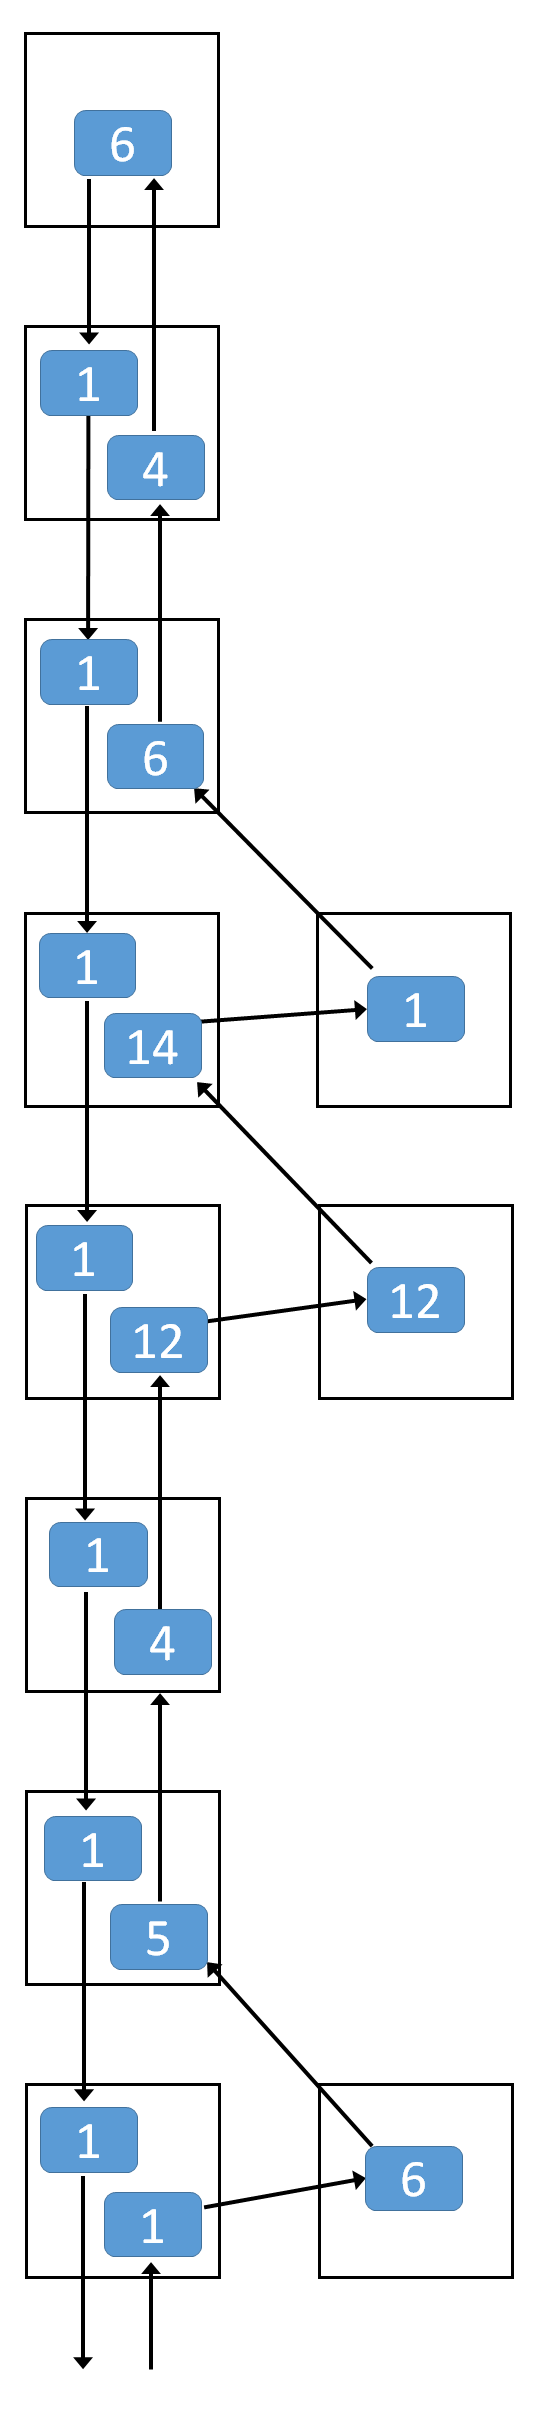
\includegraphics[scale=0.3]{./chap5/fig/1stage_data_path.eps}\\
          \hspace{2cm} (a)1ステージの場合
        \end{center}
      \end{minipage}

      % 2
      \begin{minipage}{0.5\hsize}
        \begin{center}
          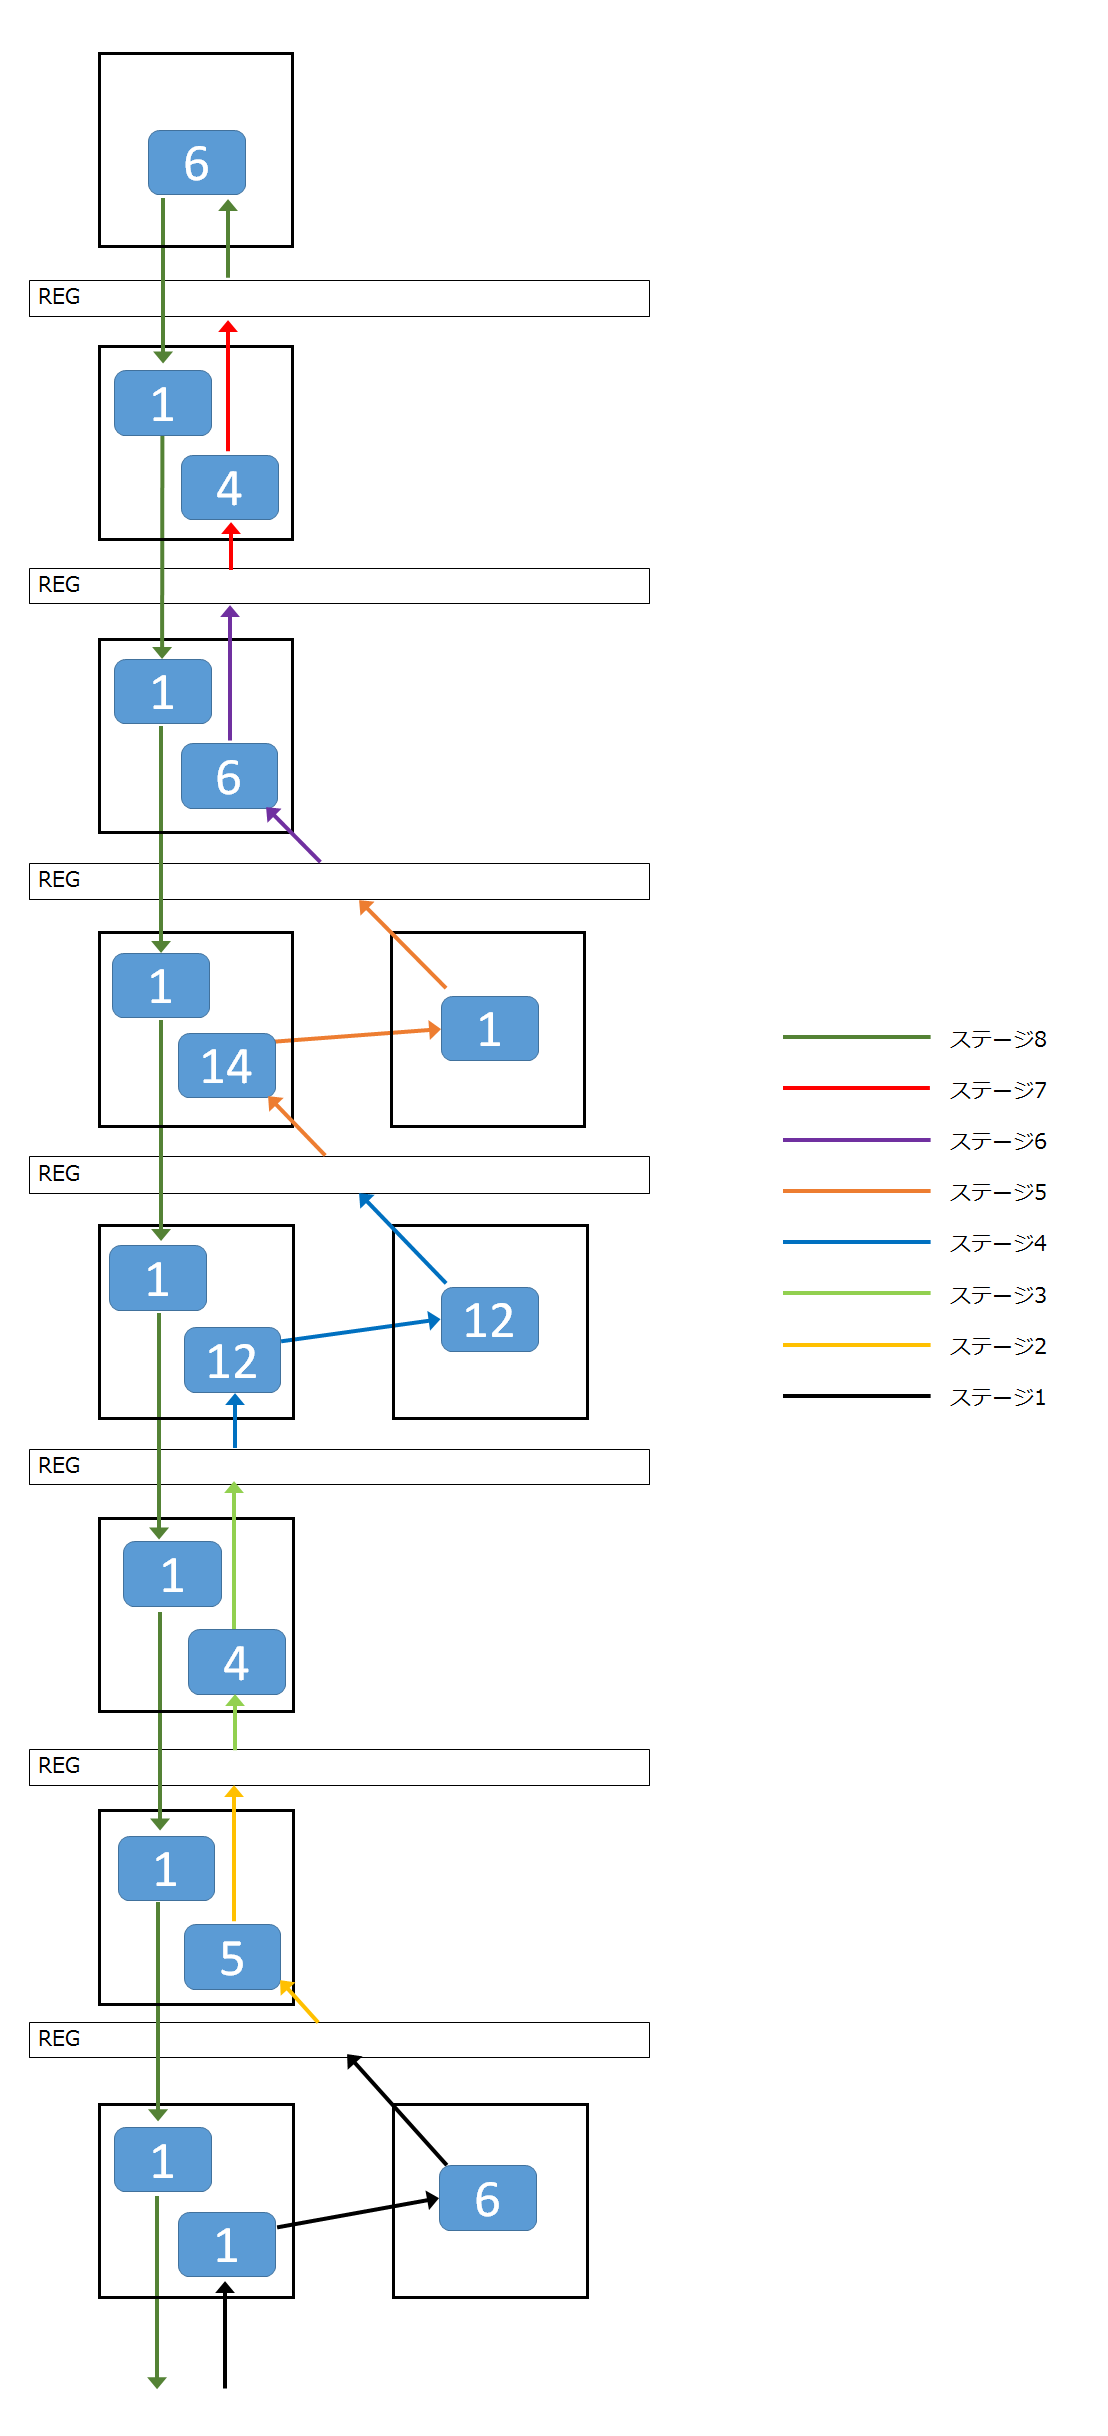
\includegraphics[scale=0.3]{./chap5/fig/8stage_data_path.eps}\\
          \hspace{2cm} (b)8ステージの場合
        \end{center}
      \end{minipage}


    \end{tabular}
    \caption{データパスと遅延の例}
    \label{fig:data_path_delay}
  \end{center}
\end{figure}

パイプライン分割しない場合の遅延時間を$D_1$とし、8段パイプラインの$n$番目のステージでの遅延を$D_8(n)$とする。これらは以下のように計算される。

\begin{eqnarray}
D_1 & = & 1 + 6 + 5 + 4 + 12 + 12 + 14 + 1 + 6 + 4 + 6 + 1 + 1 + 1 + 1 + 1 + 1 + 1 \nonumber \\
	& = & 78 \\
\nonumber \\ 
D_8(1) & = & 1 + 6 = 7 \\
D_8(2) & = &  5\\
D_8(3) & = & 4 \\
D_8(4) & = &  12 + 12 = 24 \\
D_8(5) & = &  14 + 1 = 15 \\
D_8(6) & = &  6 \\
D_8(7) & = &   4 \\
D_8(8) & = &  6 + 1 + 1 + 1 + 1 + 1 + 1 + 1 = 13
\end{eqnarray}

つまり、パイプライン分割しない1ステージの場合遅延が78であり、8ステージの場合最大遅延が24であると計算できる。


}
\chapter{まとめと今後の課題}
{
\label{chap:conclusion}
\section{結論}
\label{sec:conclusion}
VPCMAにおいて,実行するアプリケーションと要求性能に応じて電力を最小化するパイプライン段数とボディバイアス電圧を決定する手法を検討した.トレードオフの複雑さから単純に計算することが困難であったため探索はブルートフォースで行った.4つの24bit画像処理アプリケーションを実行するシミュレーションを行い評価を行った.

パイプライン段数に着目するとVPCMAおいてはアプリケーションや要求性能によらず全段にパイプライン分割した場合がもっとも電力が小さいとわかった.この結果はVPCMA特有のものであり,ブルートフォース探索によってによって明らかとなったアーキテクチャの特徴とも言える.このように本手法ではアーキテクチャに依存せずに電力を最小化するパイプライン段数を求めることができた.

ボディバイアス制御の粒度を行単位とすることによる効果をボディバイアス制御をしない場合,制御の粒度をPE\_ARRAY全体とした場合との比較を行うことにより検討した.
ボディバイアス制御をしない場合と比べて平均約46\%の電力削減率が得られた.一方で一律制御と比べると電力削減率は平均0.80\%であった.しかし,要求性能が高くなるにつれて行単位の制御では一律制御に対して高い電力削減率を示し,その効果はアプリケーションと要求性能に依存することがわかった.

\section{今後の課題}
\label{sec:future}

本論文で検討した手法にはブルートフォース探索を採用していることはすでに述べた.そのため,パイプライン分割のパターンを制限してもパイプライン段数とボディバイアス電圧を決定するのに時間がかかっていた.このようにパイプライン段数は粗粒度に探索を行っているため本研究では想定していないパイプライン分割のパターンの方がより小さい電力を示す可能性がある.ただし,本研究で示されたように電力を最小化する段数は使用している行数の付近にあるはずであり,探索はその周辺を行えばよい.よって,本論文で提案した手法のアルゴリズムには改良の余地がある.例えば遺伝的アルゴリズムなどを代表とする進化的計算アルゴリズムを採用し得られる結果と本研究のブルートフォース探索の結果を比較することにより,この手法に適するアルゴリズムを検討する必要があると考えられる.

アプリケーション依存性があるということは,どのPEにどの演算をマッピングするかに依存するということである.本研究ではアプリケーションのマッピングは固定したままでパイプライン
段数とボディバイアス電圧を変化させて電力を見積もり最小のものを探索していた.しかし,各々のパイプライン段数,ボディバイアス電圧に対する適切な演算のマッピングは異なる可能性がある.したがって,演算のマッピングを変化させた場合の影響についても評価を行う必要があると考えられる.
}

\chapter{まとめと今後の課題}
{
\label{chap:conclusion}
\section{結論}
\label{sec:conclusion}
VPCMAにおいて、実行するアプリケーションと要求性能に応じて電力を最小化するパイプライン段数とボディバイアス電圧を決定する手法を検討した。トレードオフの複雑さから単純に計算することが困難であったため探索はブルートフォースで行った。4つの24bit画像処理アプリケーションを実行するシミュレーションを行い評価を行った。

パイプライン段数に着目するとVPCMAおいてはアプリケーションや要求性能によらず全段にパイプライン分割した場合がもっとも電力が小さいとわかった。この結果はVPCMA特有のものであり、ブルートフォース探索によってによって明らかとなったアーキテクチャの特徴とも言える。このように本手法ではアーキテクチャに依存せずに電力を最小化するパイプライン段数を求めることができた。

ボディバイアス制御の粒度を行単位とすることによる効果をボディバイアス制御をしない場合、制御の粒度をPE\_ARRAY全体とした場合との比較を行うことにより検討した。
ボディバイアス制御をしない場合と比べて平均約46\%の電力削減率が得られた。一方で一律制御と比べると電力削減率は平均0.80\%であった。しかし、要求性能が高くなるにつれて行単位の制御では一律制御に対して高い電力削減率を示し、その効果はアプリケーションと要求性能に依存することがわかった。

\section{今後の課題}
\label{sec:future}

本論文で検討した手法にはブルートフォース探索を採用していることはすでに述べた。そのため、パイプライン分割のパターンを制限してもパイプライン段数とボディバイアス電圧を決定するのに時間がかかっていた。このようにパイプライン段数は粗粒度に探索を行っているため本研究では想定していないパイプライン分割のパターンの方がより小さい電力を示す可能性がある。ただし、本研究で示されたように電力を最小化する段数は使用している行数の付近にあるはずであり、探索はその周辺を行えばよい。よって、本論文で提案した手法のアルゴリズムには改良の余地がある。例えば遺伝的アルゴリズムなどを代表とする進化的計算アルゴリズムを採用し得られる結果と本研究のブルートフォース探索の結果を比較することにより、この手法に適するアルゴリズムを検討する必要があると考えられる。

アプリケーション依存性があるということは、どのPEにどの演算をマッピングするかに依存するということである。本研究ではアプリケーションのマッピングは固定したままでパイプライン
段数とボディバイアス電圧を変化させて電力を見積もり最小のものを探索していた。しかし、各々のパイプライン段数、ボディバイアス電圧に対する適切な演算のマッピングは異なる可能性がある。したがって、演算のマッピングを変化させた場合の影響についても評価を行う必要があると考えられる。
}

\chapter{謝辞}
{
本研究に取り組むにあたりご指導ご鞭撻を賜りました天野英晴教授,に深く感謝いたします.
主査をしていただくとともにVivadoの使い方、アクセラレータ実装での助言を頂いた武者千嵯氏、副査として
論文の基本的な書き方を教授してくださった安戸僚汰氏にも深く感謝いたします。

}

%-end body-----------------------------------------%


%-reference----------------------------------------%
\bibliographystyle{junsrt}
%\nocites{*}
\bibliography{bibdata}
%-end reference------------------------------------%
\end{document}
